\documentclass[11pt,a4paper]{article}
% ============================================================
% Shared preamble for Claude Experiments reports (pdflatex)
% Include this AFTER \documentclass in each report:
%   \documentclass[11pt,a4paper]{article}
%   % ============================================================
% Shared preamble for Claude Experiments reports (pdflatex)
% Include this AFTER \documentclass in each report:
%   \documentclass[11pt,a4paper]{article}
%   % ============================================================
% Shared preamble for Claude Experiments reports (pdflatex)
% Include this AFTER \documentclass in each report:
%   \documentclass[11pt,a4paper]{article}
%   \input{../preamble}
% ============================================================
\usepackage[T1]{fontenc}
\usepackage[utf8]{inputenc}
\usepackage[english]{babel}
\usepackage[a4paper,top=2.5cm,bottom=2.5cm,left=2.5cm,right=2.5cm]{geometry}
\usepackage{amsmath,amssymb}
\usepackage{graphicx}
\usepackage{subcaption}
\usepackage{booktabs}
\usepackage{xcolor}
\usepackage[colorlinks=true,allcolors=blue]{hyperref}
\usepackage{microtype}
\usepackage{float}
\usepackage{array}
\microtypesetup{expansion=false}

% Color scheme
\definecolor{colMicro}{HTML}{222222}
\definecolor{colExact}{HTML}{2878b5}
\definecolor{colPlacement}{HTML}{e07a1f}
\definecolor{colBoundary}{HTML}{429c74}
\definecolor{colCurrent}{HTML}{c23b55}
\definecolor{colMM}{HTML}{c23b55}

\providecommand{\SIG}{\textcolor{green!50!black}{\textbf{*}}}
\providecommand{\NS}{\textcolor{gray}{n.s.}}
\providecommand{\DRMS}{\Delta\mathrm{RMST}}
\providecommand{\ci}[2]{$[{#1},\;{#2}]$}

% ============================================================
\usepackage[T1]{fontenc}
\usepackage[utf8]{inputenc}
\usepackage[english]{babel}
\usepackage[a4paper,top=2.5cm,bottom=2.5cm,left=2.5cm,right=2.5cm]{geometry}
\usepackage{amsmath,amssymb}
\usepackage{graphicx}
\usepackage{subcaption}
\usepackage{booktabs}
\usepackage{xcolor}
\usepackage[colorlinks=true,allcolors=blue]{hyperref}
\usepackage{microtype}
\usepackage{float}
\usepackage{array}
\microtypesetup{expansion=false}

% Color scheme
\definecolor{colMicro}{HTML}{222222}
\definecolor{colExact}{HTML}{2878b5}
\definecolor{colPlacement}{HTML}{e07a1f}
\definecolor{colBoundary}{HTML}{429c74}
\definecolor{colCurrent}{HTML}{c23b55}
\definecolor{colMM}{HTML}{c23b55}

\providecommand{\SIG}{\textcolor{green!50!black}{\textbf{*}}}
\providecommand{\NS}{\textcolor{gray}{n.s.}}
\providecommand{\DRMS}{\Delta\mathrm{RMST}}
\providecommand{\ci}[2]{$[{#1},\;{#2}]$}

% ============================================================
\usepackage[T1]{fontenc}
\usepackage[utf8]{inputenc}
\usepackage[english]{babel}
\usepackage[a4paper,top=2.5cm,bottom=2.5cm,left=2.5cm,right=2.5cm]{geometry}
\usepackage{amsmath,amssymb}
\usepackage{graphicx}
\usepackage{subcaption}
\usepackage{booktabs}
\usepackage{xcolor}
\usepackage[colorlinks=true,allcolors=blue]{hyperref}
\usepackage{microtype}
\usepackage{float}
\usepackage{array}
\microtypesetup{expansion=false}

% Color scheme
\definecolor{colMicro}{HTML}{222222}
\definecolor{colExact}{HTML}{2878b5}
\definecolor{colPlacement}{HTML}{e07a1f}
\definecolor{colBoundary}{HTML}{429c74}
\definecolor{colCurrent}{HTML}{c23b55}
\definecolor{colMM}{HTML}{c23b55}

\providecommand{\SIG}{\textcolor{green!50!black}{\textbf{*}}}
\providecommand{\NS}{\textcolor{gray}{n.s.}}
\providecommand{\DRMS}{\Delta\mathrm{RMST}}
\providecommand{\ci}[2]{$[{#1},\;{#2}]$}

\title{CE-06: Parameter Regime Map of MicroMacro Error}
\author{Two-Layer CTMC Experiments Pipeline}
\date{August 4, 2026}
\begin{document}\maketitle
\begin{abstract}
CE-06 maps terminal-arrival error over export ratio $r$, internal degree $d$, and interface width $k$. The 36-cell, 60-replication study shows that error is not a fixed premature-arrival offset: its sign and magnitude depend strongly on the competition between export and internal mixing. Faster export and sparse communities produce the largest premature bias, whereas slow export in dense communities can produce late bias. This rules out an always-on damping correction and motivates a regime-aware gate.
\end{abstract}

\section{Design and estimand}
Each cell used a chain of ten connected random communities, $n=100$, $\beta_{in}=0.003$, $r=\beta_{out}/\beta_{in}\in\{0.5,1,2\}$, $d\in\{4,6,10,20\}$, and $k\in\{2,5,10\}$. Sixty paired network/initialization replications were run per cell. Horizons were chosen per cell; therefore the primary cross-cell estimand is $\Delta\mathrm{RMST}/T_{end}$, while completion differences flag residual censoring.

\section{Results}
\begin{table}[H]\centering
\caption{Mean normalized error over the twelve $(d,k)$ cells at each export ratio.}
\begin{tabular}{rrrrr}\toprule
$r$ & Mean & Cell minimum & Cell maximum & Mean rel-$W_1$\\\midrule
0.5 & -0.0028 & -0.0638 & 0.1132 & 0.241\\
1.0 & -0.1275 & -0.2765 & -0.0495 & 0.348\\
2.0 & -0.3034 & -0.5281 & -0.1510 & 0.543\\
\bottomrule\end{tabular}
\end{table}
Bootstrap intervals excluded zero in 34 of 36 cells. Averaged over $r$ and $k$, normalized error moved from $-0.222$ at $d=4$ to $-0.075$ at $d=20$. Averaged over $r$ and $d$, it moved from $-0.176$ at $k=2$ to $-0.115$ at $k=10$. The most premature cell was $(r,d,k)=(2,4,2)$ at $-0.528$; the largest late cell was $(0.5,20,2)$ at $+0.113$.

\begin{figure}[H]\centering
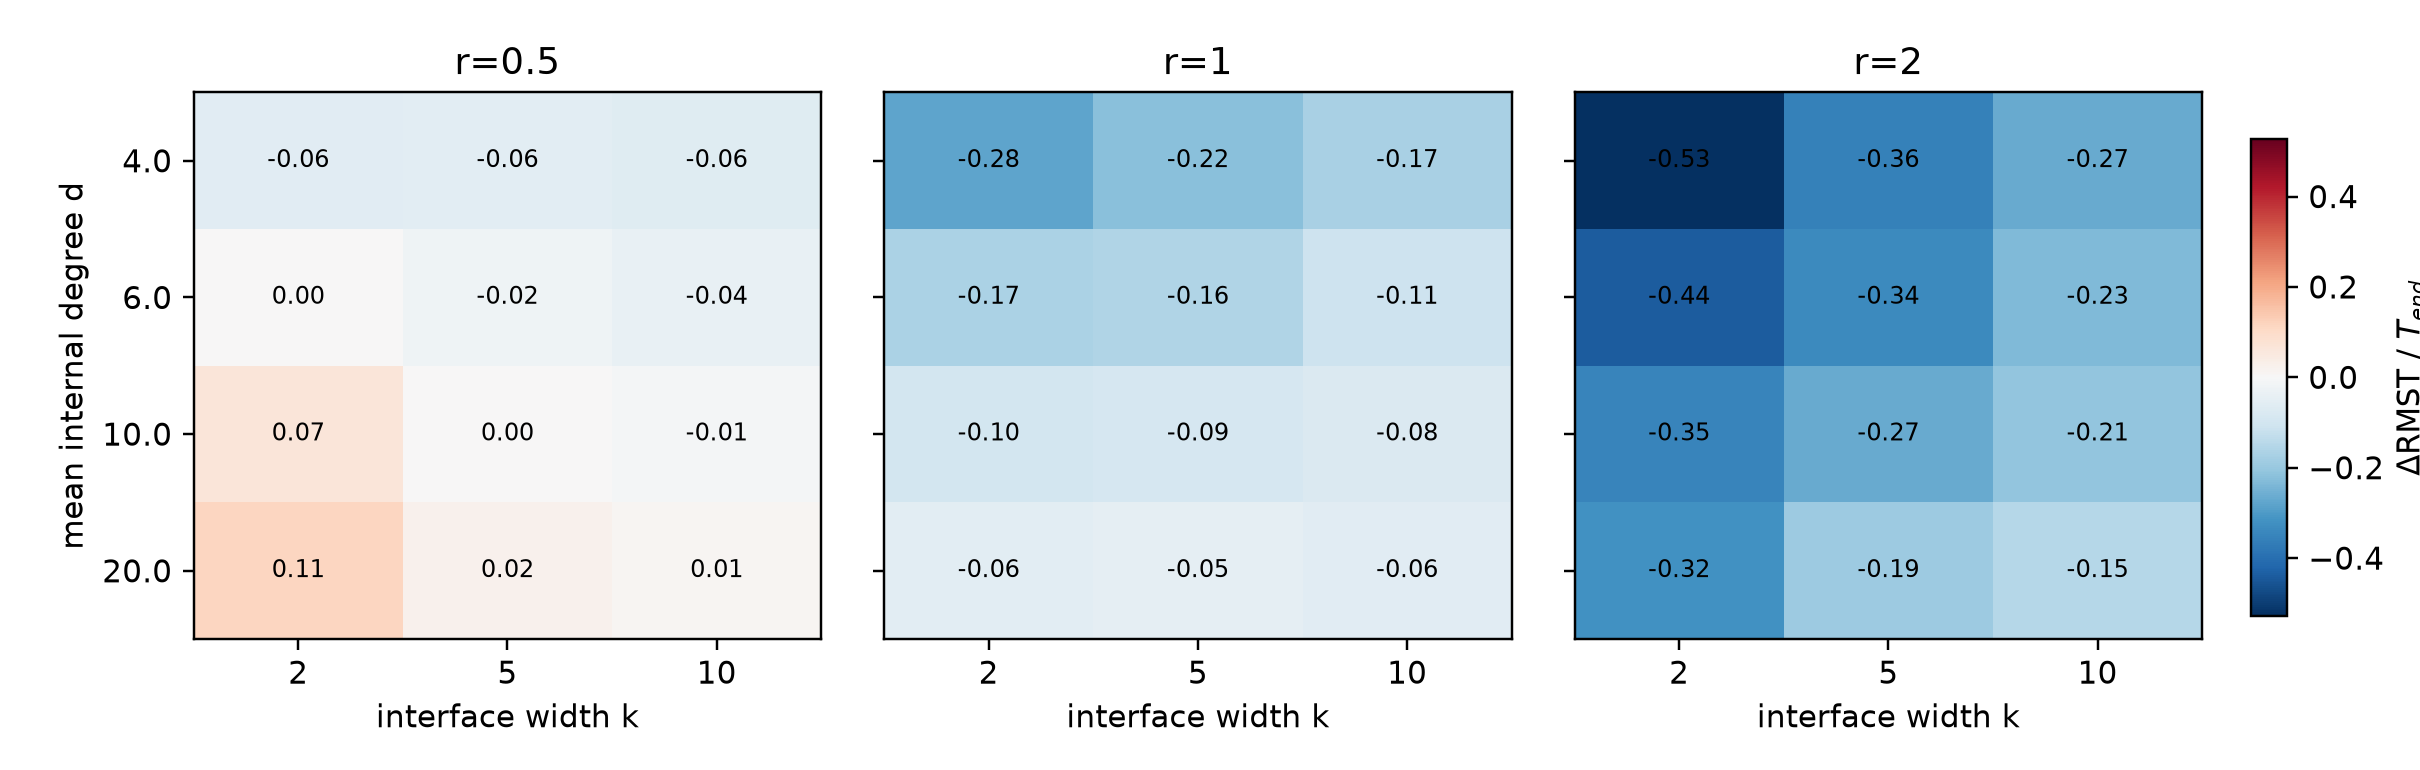
\includegraphics[width=.98\linewidth]{figures/regime_map.png}
\caption{Normalized RMST difference. Each number summarizes 60 independent paired replications; colors are centered at zero.}
\end{figure}

\section{Implications for reducing the error}
The export ratio is the dominant design variable in this grid. Low degree and narrow interfaces amplify premature leakage because aggregate prevalence becomes positive before infection reaches a small gateway set. Increasing $d$ or $k$ reduces this mismatch but does not remove it at $r\ge1$.

An unconditional reduction of macro hazard is scientifically unsafe: at $r=0.5$ the baseline error crosses zero and becomes late in dense cells, so further damping must worsen those cells. A viable correction must therefore (i) strengthen with $r$ relative to a mixing descriptor, (ii) self-disable in dense or broad-interface regimes, and (iii) permit no correction, rather than forced damping, near the empirical sign boundary. CE-06 supports fitting or validating such a gate, but it does not itself identify a causal formula because $d$, spectral statistics, and boundary accessibility covary.

\section{Limitations and consequence}
The study is SI-only and uses one random-connected topology family. Adaptive horizons make raw RMST incomparable across cells, and four high-$r$, $k=2$ cells retain completion differences. The practical consequence is that candidate corrections must be evaluated on normalized censoring-aware metrics and across topology, not selected from one baseline.

\section*{Reproduction}
\texttt{.venv/bin/python extrascripts/run\_ce06\_regime\_map.py --grid full --workers 8 --resume}
\end{document}
